% \documentclass[aspectratio=169,notes]{beamer}
\documentclass[aspectratio=169]{beamer}
\usetheme[faculty=phil]{fibeamer}
\usepackage{polyglossia}
\setmainlanguage{english} %% main locale instead of `english`, you
%% can typeset the presentation in either Czech or Slovak,
%% respectively.
\setotherlanguages{russian} %% The additional keys allow
%%
%%   \begin{otherlanguage}{czech}   ... \end{otherlanguage}
%%   \begin{otherlanguage}{slovak}  ... \end{otherlanguage}
%%
%% These macros specify information about the presentation
\title[Theoretical Mechanics]{Week HW 6, COM LINEAR ANGULAR} %% that will be typeset on the
\subtitle{Motion of the centre of mass of a system\\
Change of Principal Angular momentum of a system\\
\ 
         } %% title page.
\author{Oleg Bulichev}
%% These additional packages are used within the document:
\usepackage{ragged2e}  % `\justifying` text
\usepackage{booktabs}  % Tables
\usepackage{tabularx}
\usepackage{tikz}      % Diagrams
\usetikzlibrary{calc, shapes, backgrounds}
\usepackage{amsmath, amssymb}
\usepackage{url}       % `\url`s
\usepackage{listings}  % Code listings
% \usepackage{subfigure}
\usepackage{floatrow}
\usepackage{subcaption}
\usepackage{mathtools}
\usepackage{todonotes}
\usepackage{fontspec}
\usepackage{multicol}
\usepackage{pdfpages}
\usepackage{wrapfig}
\usepackage{animate}
\usepackage{booktabs}
\usepackage{multirow}
% \usepackage{graphicx}
\usepackage{colortbl}

\graphicspath{{resources/}}
\frenchspacing

\setbeamertemplate{caption}[numbered]
\usetikzlibrary{graphs}

% \usepackage[backend=biber,style=ieee,autocite=footnote]{biblatex}
% \addbibresource{biblio.bib}
% \DefineBibliographyStrings{english}{%
%   bibliography = {References},}

\newcommand{\oleg}[2][] {\todo[color=red, #1] {OLEG:\\ #2}}
\newcommand{\fbckg}[1]{\usebackgroundtemplate{\includegraphics[width=\paperwidth]{#1}}}%frame background

\usepackage[framemethod=TikZ]{mdframed}
\newcommand{\dbox}[1]{
\begin{mdframed}[roundcorner=3pt, backgroundcolor=yellow, linewidth=0]
\vspace{1mm}
{#1}
\vspace{1mm}
\end{mdframed}
}

\begin{document}
\setlength{\abovedisplayskip}{0pt}
\setlength{\belowdisplayskip}{0pt}
\setlength{\abovedisplayshortskip}{0pt}
\setlength{\belowdisplayshortskip}{0pt}

\fbckg{fibeamer/figs/title_page.png}
\frame[c]{\setcounter{framenumber}{0}
    \usebeamerfont{title}%
    \usebeamercolor[fg]{title}%
    \begin{minipage}[b][6.5\baselineskip][b]{\textwidth}%
        \textcolor{black}{\raggedright\inserttitle}
    \end{minipage}
    % \vskip-1.5\baselineskip

    \usebeamerfont{subtitle}%
    \usebeamercolor[fg]{framesubtitle}%
    \begin{minipage}[b][3\baselineskip][b]{\textwidth}
        \raggedright%
        \insertsubtitle%
    \end{minipage}
    \vskip.25\baselineskip
}
%   \frame[c]{\maketitle}

\fbckg{fibeamer/figs/common.png}


\begin{frame}[t]{Task 1}
  \begin{minipage}{0.6\textwidth}
    There are 3 weights with masses $M_1=20\ kg,\ M_2=15\ kg,\ M_3=10\ kg$. They are connected by ideal string. This string go through by two pulleys $L,\ N$. When the $M_1$ weight goes down on $1\ meter$, the body $ABCD$ shifts on some distance $S$.

    The task is to find the distance of this movement according to the ground. Neglect the friction between the floor and $ABCD$. \smallskip
    
    \textit{Answer}: It will move to the left on $14$ cm.
  \end{minipage}
  \begin{minipage}{0.39\textwidth}
    \begin{figure}[H]
      \centering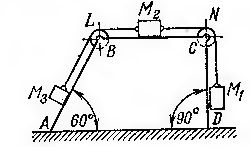
\includegraphics[height=6cm,width=1\textwidth,keepaspectratio]{HW5_3}
      \caption*{Task 1}
    \end{figure}
  \end{minipage}
\end{frame}

\begin{frame}[t]{Task 2}
  \begin{minipage}{0.6\textwidth}
    On the figure a pulley with a rope running over it is presented. A man (mass $m$) holds one side of the rope at $A$ while a load, equal to the weight of the man, is attached to the other end of the rope at $B$.
    
    What would happen to the load if the man starts climbing up the rope with the velocity $a$ relative to the rope.

    The weight of the pulley is equal $0.25$. The mass of the pulley is distributed uniformly along its rim. \smallskip

    \textit{Answer}: The load will ascend with velocity $\dfrac{4}{9}a$.
  \end{minipage}
  \begin{minipage}{0.39\textwidth}
    \begin{figure}[H]
      \centering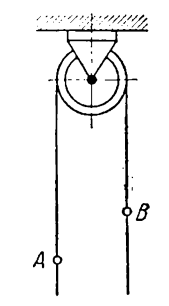
\includegraphics[height=5cm,width=1\textwidth,keepaspectratio]{HW6_1}
      \caption*{Task 2}
    \end{figure}
  \end{minipage}
\end{frame}

\fbckg{fibeamer/figs/last_page.png}
\frame[plain]{}
\end{document}